\section{moeo\-Binary\-Hypervolume\-Indicator$<$ EOFitness $>$ Class Template Reference}
\label{classmoeoBinaryHypervolumeIndicator}\index{moeoBinaryHypervolumeIndicator@{moeoBinaryHypervolumeIndicator}}
Functor Binary hypervolume indicator for {\bf eo\-Pareto\-Fitness}.  


{\tt \#include $<$moeo\-Binary\-Quality\-Indicator.h$>$}

Inheritance diagram for moeo\-Binary\-Hypervolume\-Indicator$<$ EOFitness $>$::\begin{figure}[H]
\begin{center}
\leavevmode
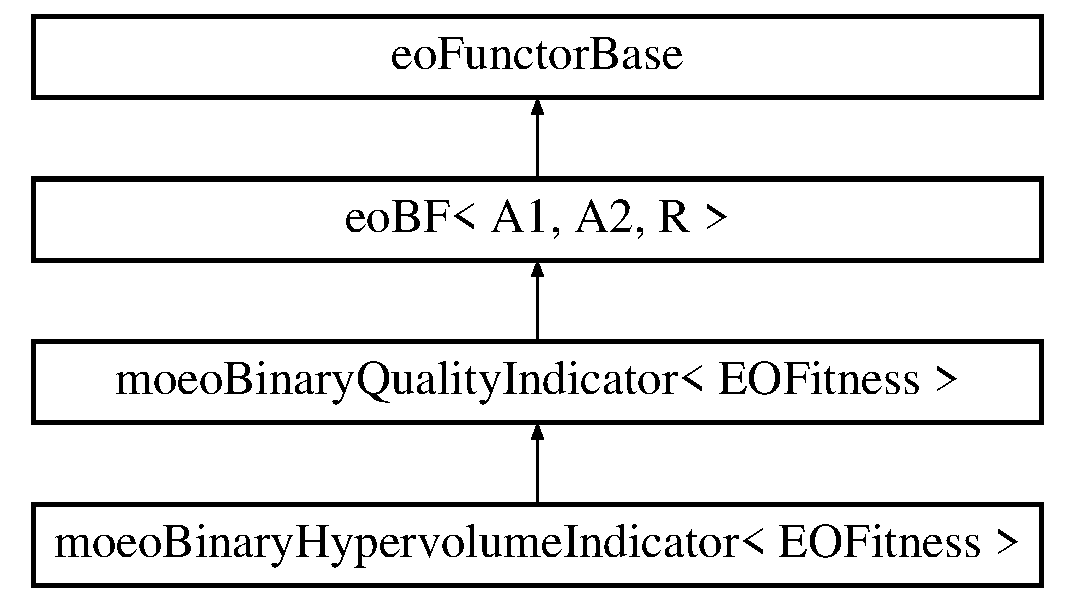
\includegraphics[height=4cm]{classmoeoBinaryHypervolumeIndicator}
\end{center}
\end{figure}
\subsection*{Public Member Functions}
\begin{CompactItemize}
\item 
{\bf moeo\-Binary\-Hypervolume\-Indicator} (double \_\-rho)
\begin{CompactList}\small\item\em constructor \item\end{CompactList}\item 
double {\bf operator()} (const EOFitness \&\_\-fitness\_\-eo1, const EOFitness \&\_\-fitness\_\-eo2)
\begin{CompactList}\small\item\em indicator value of the hypervolume of the portion of the objective space that is dominated by individual \_\-eo1 but not by individual \_\-eo2 (don't forget to set the bounds before the call of this function) \item\end{CompactList}\end{CompactItemize}
\subsection*{Private Types}
\begin{CompactItemize}
\item 
typedef EOFitness::fitness\_\-traits {\bf traits}\label{classmoeoBinaryHypervolumeIndicator_511931936ec9e368b5f0cbcdc4dbe020}

\begin{CompactList}\small\item\em fitness traits \item\end{CompactList}\end{CompactItemize}
\subsection*{Private Member Functions}
\begin{CompactItemize}
\item 
double {\bf hypervolume\-Indicator\-Value} (const EOFitness \&\_\-fitness\_\-eo1, const EOFitness \&\_\-fitness\_\-eo2, const unsigned \_\-i\-Obj, const bool \_\-flag=false)
\begin{CompactList}\small\item\em computation of the hypervolume of the portion of the objective space that is dominated by individual \_\-eo1 but not by individual \_\-eo2 \item\end{CompactList}\item 
double {\bf hypervolume\-Indicator\-Value\-Min} (const EOFitness \&\_\-fitness\_\-eo1, const EOFitness \&\_\-fitness\_\-eo2, const unsigned \_\-i\-Obj, const bool \_\-flag)
\begin{CompactList}\small\item\em computation of the hypervolume of the portion of the objective space that is dominated by individual \_\-eo1 but not by individual \_\-eo2 in case of a minimization on the objective \_\-i\-Obj \item\end{CompactList}\item 
double {\bf hypervolume\-Indicator\-Value\-Max} (const EOFitness \&\_\-fitness\_\-eo1, const EOFitness \&\_\-fitness\_\-eo2, const unsigned \_\-i\-Obj, const bool \_\-flag)
\begin{CompactList}\small\item\em computation of the hypervolume of the portion of the objective space that is dominated by individual \_\-eo1 but not by individual \_\-eo2 in case of a maximization on the objective \_\-i\-Obj \item\end{CompactList}\end{CompactItemize}
\subsection*{Private Attributes}
\begin{CompactItemize}
\item 
double {\bf rho}\label{classmoeoBinaryHypervolumeIndicator_06b7c3ba8fa0ceafd7e6b571e43e6f4c}

\begin{CompactList}\small\item\em reference point for the hypervolume calculation \item\end{CompactList}\end{CompactItemize}


\subsection{Detailed Description}
\subsubsection*{template$<$class EOFitness$>$ class moeo\-Binary\-Hypervolume\-Indicator$<$ EOFitness $>$}

Functor Binary hypervolume indicator for {\bf eo\-Pareto\-Fitness}. 



Definition at line 206 of file moeo\-Binary\-Quality\-Indicator.h.

\subsection{Constructor \& Destructor Documentation}
\index{moeoBinaryHypervolumeIndicator@{moeo\-Binary\-Hypervolume\-Indicator}!moeoBinaryHypervolumeIndicator@{moeoBinaryHypervolumeIndicator}}
\index{moeoBinaryHypervolumeIndicator@{moeoBinaryHypervolumeIndicator}!moeoBinaryHypervolumeIndicator@{moeo\-Binary\-Hypervolume\-Indicator}}
\subsubsection{\setlength{\rightskip}{0pt plus 5cm}template$<$class EOFitness$>$ {\bf moeo\-Binary\-Hypervolume\-Indicator}$<$ EOFitness $>$::{\bf moeo\-Binary\-Hypervolume\-Indicator} (double {\em \_\-rho})\hspace{0.3cm}{\tt  [inline]}}\label{classmoeoBinaryHypervolumeIndicator_15d486d524816d294bc007d7a555cbfe}


constructor 

\begin{Desc}
\item[Parameters:]
\begin{description}
\item[{\em double}]\_\-rho reference point for the hypervolume calculation (rho must not be smaller than 1) \end{description}
\end{Desc}


Definition at line 216 of file moeo\-Binary\-Quality\-Indicator.h.

References moeo\-Binary\-Hypervolume\-Indicator$<$ EOFitness $>$::rho.

\subsection{Member Function Documentation}
\index{moeoBinaryHypervolumeIndicator@{moeo\-Binary\-Hypervolume\-Indicator}!operator()@{operator()}}
\index{operator()@{operator()}!moeoBinaryHypervolumeIndicator@{moeo\-Binary\-Hypervolume\-Indicator}}
\subsubsection{\setlength{\rightskip}{0pt plus 5cm}template$<$class EOFitness$>$ double {\bf moeo\-Binary\-Hypervolume\-Indicator}$<$ EOFitness $>$::operator() (const EOFitness \& {\em \_\-fitness\_\-eo1}, const EOFitness \& {\em \_\-fitness\_\-eo2})\hspace{0.3cm}{\tt  [inline]}}\label{classmoeoBinaryHypervolumeIndicator_697e7fcab99f5192925e2f2157d1e1a3}


indicator value of the hypervolume of the portion of the objective space that is dominated by individual \_\-eo1 but not by individual \_\-eo2 (don't forget to set the bounds before the call of this function) 

\begin{Desc}
\item[Parameters:]
\begin{description}
\item[{\em EOFitness}]\& \_\-fitness\_\-eo1 the fitness of the first individual \item[{\em EOFitness}]\& \_\-fitness\_\-eo2 the fitness of the second individual \end{description}
\end{Desc}


Definition at line 239 of file moeo\-Binary\-Quality\-Indicator.h.

References moeo\-Binary\-Hypervolume\-Indicator$<$ EOFitness $>$::hypervolume\-Indicator\-Value().\index{moeoBinaryHypervolumeIndicator@{moeo\-Binary\-Hypervolume\-Indicator}!hypervolumeIndicatorValue@{hypervolumeIndicatorValue}}
\index{hypervolumeIndicatorValue@{hypervolumeIndicatorValue}!moeoBinaryHypervolumeIndicator@{moeo\-Binary\-Hypervolume\-Indicator}}
\subsubsection{\setlength{\rightskip}{0pt plus 5cm}template$<$class EOFitness$>$ double {\bf moeo\-Binary\-Hypervolume\-Indicator}$<$ EOFitness $>$::hypervolume\-Indicator\-Value (const EOFitness \& {\em \_\-fitness\_\-eo1}, const EOFitness \& {\em \_\-fitness\_\-eo2}, const unsigned {\em \_\-i\-Obj}, const bool {\em \_\-flag} = {\tt false})\hspace{0.3cm}{\tt  [inline, private]}}\label{classmoeoBinaryHypervolumeIndicator_dd0c63a922cb4bf921978413fdb1dca0}


computation of the hypervolume of the portion of the objective space that is dominated by individual \_\-eo1 but not by individual \_\-eo2 

\begin{Desc}
\item[Parameters:]
\begin{description}
\item[{\em EOFitness}]\& \_\-fitness\_\-eo1 the fitness of the first individual \item[{\em EOFitness}]\& \_\-fitness\_\-eo2 the fitness of the second individual \item[{\em unsigned}]\_\-i\-Obj number of objectives (used for iteration) \item[{\em bool}]\_\-flag = false (only used for iteration) \end{description}
\end{Desc}


Definition at line 274 of file moeo\-Binary\-Quality\-Indicator.h.

References moeo\-Binary\-Quality\-Indicator$<$ EOFitness $>$::bounds, moeo\-Binary\-Hypervolume\-Indicator$<$ EOFitness $>$::hypervolume\-Indicator\-Value\-Max(), and moeo\-Binary\-Hypervolume\-Indicator$<$ EOFitness $>$::hypervolume\-Indicator\-Value\-Min().

Referenced by moeo\-Binary\-Hypervolume\-Indicator$<$ EOFitness $>$::hypervolume\-Indicator\-Value\-Max(), moeo\-Binary\-Hypervolume\-Indicator$<$ EOFitness $>$::hypervolume\-Indicator\-Value\-Min(), and moeo\-Binary\-Hypervolume\-Indicator$<$ EOFitness $>$::operator()().\index{moeoBinaryHypervolumeIndicator@{moeo\-Binary\-Hypervolume\-Indicator}!hypervolumeIndicatorValueMin@{hypervolumeIndicatorValueMin}}
\index{hypervolumeIndicatorValueMin@{hypervolumeIndicatorValueMin}!moeoBinaryHypervolumeIndicator@{moeo\-Binary\-Hypervolume\-Indicator}}
\subsubsection{\setlength{\rightskip}{0pt plus 5cm}template$<$class EOFitness$>$ double {\bf moeo\-Binary\-Hypervolume\-Indicator}$<$ EOFitness $>$::hypervolume\-Indicator\-Value\-Min (const EOFitness \& {\em \_\-fitness\_\-eo1}, const EOFitness \& {\em \_\-fitness\_\-eo2}, const unsigned {\em \_\-i\-Obj}, const bool {\em \_\-flag})\hspace{0.3cm}{\tt  [inline, private]}}\label{classmoeoBinaryHypervolumeIndicator_637f559f83f473412c61d4a485af5993}


computation of the hypervolume of the portion of the objective space that is dominated by individual \_\-eo1 but not by individual \_\-eo2 in case of a minimization on the objective \_\-i\-Obj 

\begin{Desc}
\item[Parameters:]
\begin{description}
\item[{\em EOFitness}]\& \_\-fitness\_\-eo1 the fitness of the first individual \item[{\em EOFitness}]\& \_\-fitness\_\-eo2 the fitness of the second individual \item[{\em unsigned}]\_\-i\-Obj index of the objective \item[{\em bool}]\_\-flag (only used for iteration) \end{description}
\end{Desc}


Definition at line 309 of file moeo\-Binary\-Quality\-Indicator.h.

References moeo\-Binary\-Quality\-Indicator$<$ EOFitness $>$::bounds, moeo\-Binary\-Hypervolume\-Indicator$<$ EOFitness $>$::hypervolume\-Indicator\-Value(), and moeo\-Binary\-Hypervolume\-Indicator$<$ EOFitness $>$::rho.

Referenced by moeo\-Binary\-Hypervolume\-Indicator$<$ EOFitness $>$::hypervolume\-Indicator\-Value().\index{moeoBinaryHypervolumeIndicator@{moeo\-Binary\-Hypervolume\-Indicator}!hypervolumeIndicatorValueMax@{hypervolumeIndicatorValueMax}}
\index{hypervolumeIndicatorValueMax@{hypervolumeIndicatorValueMax}!moeoBinaryHypervolumeIndicator@{moeo\-Binary\-Hypervolume\-Indicator}}
\subsubsection{\setlength{\rightskip}{0pt plus 5cm}template$<$class EOFitness$>$ double {\bf moeo\-Binary\-Hypervolume\-Indicator}$<$ EOFitness $>$::hypervolume\-Indicator\-Value\-Max (const EOFitness \& {\em \_\-fitness\_\-eo1}, const EOFitness \& {\em \_\-fitness\_\-eo2}, const unsigned {\em \_\-i\-Obj}, const bool {\em \_\-flag})\hspace{0.3cm}{\tt  [inline, private]}}\label{classmoeoBinaryHypervolumeIndicator_c0a602a4f1a27418d95d883f53e45cb2}


computation of the hypervolume of the portion of the objective space that is dominated by individual \_\-eo1 but not by individual \_\-eo2 in case of a maximization on the objective \_\-i\-Obj 

\begin{Desc}
\item[Parameters:]
\begin{description}
\item[{\em EOFitness}]\& \_\-fitness\_\-eo1 the fitness of the first individual \item[{\em EOFitness}]\& \_\-fitness\_\-eo2 the fitness of the second individual \item[{\em unsigned}]\_\-i\-Obj index of the objective \item[{\em bool}]\_\-flag (only used for iteration) \end{description}
\end{Desc}


Definition at line 363 of file moeo\-Binary\-Quality\-Indicator.h.

References moeo\-Binary\-Quality\-Indicator$<$ EOFitness $>$::bounds, moeo\-Binary\-Hypervolume\-Indicator$<$ EOFitness $>$::hypervolume\-Indicator\-Value(), and moeo\-Binary\-Hypervolume\-Indicator$<$ EOFitness $>$::rho.

Referenced by moeo\-Binary\-Hypervolume\-Indicator$<$ EOFitness $>$::hypervolume\-Indicator\-Value().

The documentation for this class was generated from the following file:\begin{CompactItemize}
\item 
moeo\-Binary\-Quality\-Indicator.h\end{CompactItemize}
